\documentclass[a4paper,12pt]{extarticle}

%% Language and font encodings
\usepackage[english]{babel}
\usepackage[utf8x]{inputenc}
\usepackage[T1]{fontenc}

%% Sets page size and margins
\usepackage[a4paper,top=3cm,bottom=2cm,left=3cm,right=3cm,marginparwidth=1.75cm]{geometry}

%% Useful packages
\usepackage{amsmath}
\usepackage{graphicx}
\usepackage[colorinlistoftodos]{todonotes}
\usepackage[colorlinks=true, allcolors=blue]{hyperref}

\title{ENERGY 294 Homework 3}
\author{Sam Kramer}

\begin{document}

\maketitle

\section{Problem 1}

\subsection{}

\begin{figure}[h]
\centering
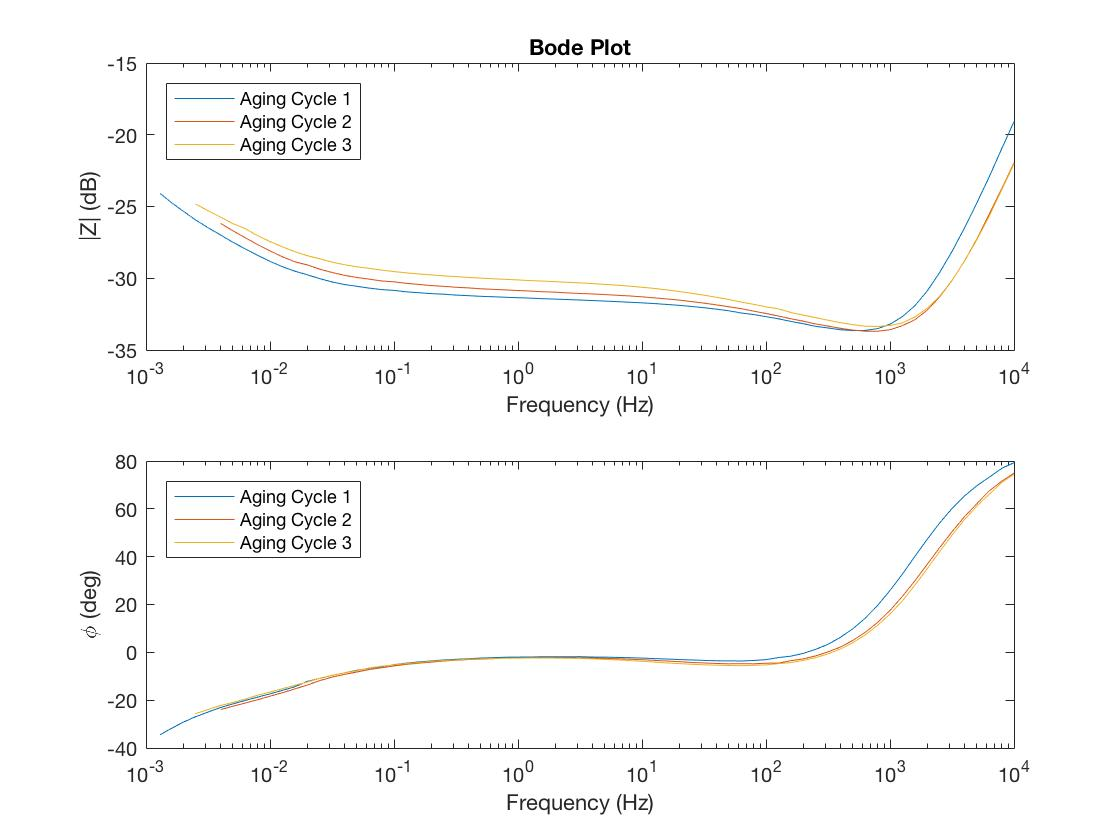
\includegraphics[width=\textwidth]{bode.jpg}
\end{figure}

\begin{figure}[h]
\centering
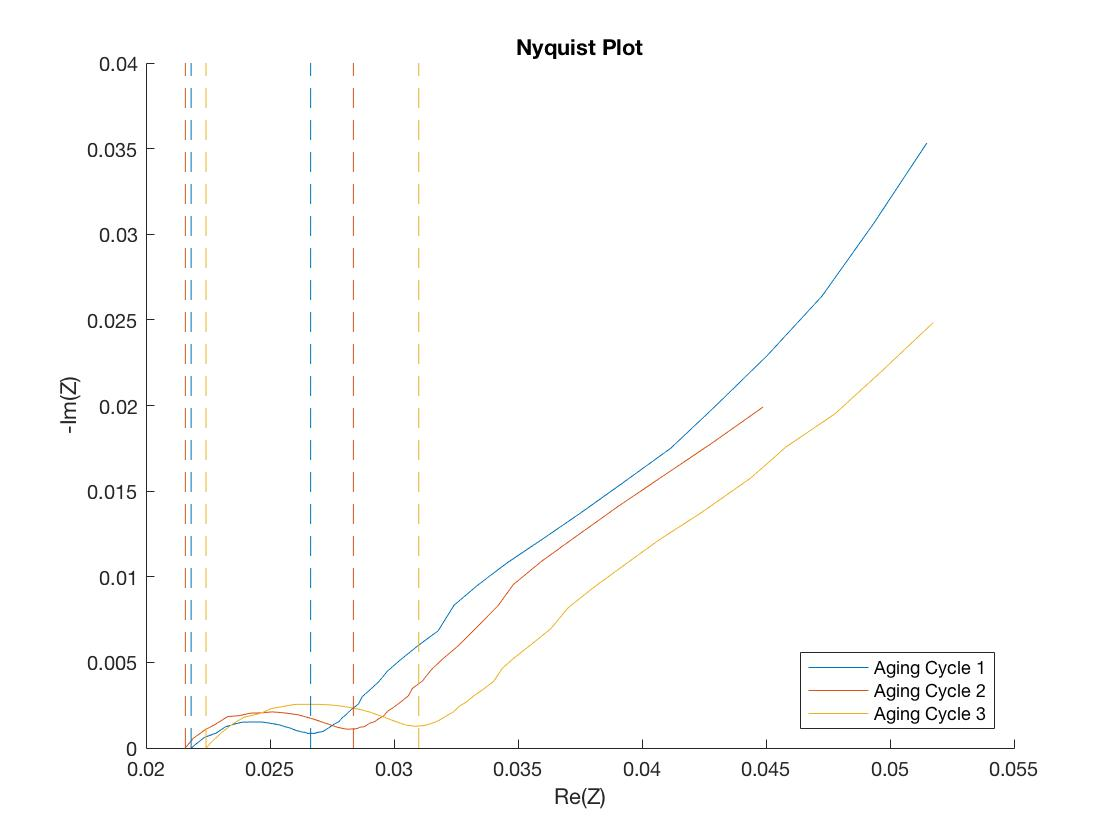
\includegraphics[width=\textwidth]{nyquist.jpg}
\end{figure}

\pagebreak

\subsection{}

The leftmost vertical reference lines on Nyquist plot represent the intersection of each curve with the real axis. The distance along the x-axis from (0,0) to these x-coordinates represent \(R_E\), the resistance due to the battery electrolyte. The rightmost vertical reference lines represent the dips in each curve that occur before the linear behavior starts. The distance between each leftmost vertical reference line and its corresponding rightmost vertical line represents \(R_{CT}\), the charge transfer resistance. The imaginary component of the impedance between these reference lines is the contribution of \(C_{DL}\), the double layer capacitance, since resistors have no imaginary impedance and capacitors have only imaginary impedance. The portion of the curve to the right of \(R_E\) + \(R_{CT}\), which appears to be roughly linear, represents the Warburg impedance, \(R_W\). 

\subsection{}

As the aging state of the cell increases, \(R_E\) seems to increase slightly, although there appears in this dataset to be a slight decrease in \(R_E\) between aging cycle 1 and aging cycle 2. \(R_{CT}\), on the other hand, increases much more with the aging cycles. This increase in \(R_E\) and/or \(R_{CT}\) could possibly be due to the buildup of solid-electrolyte interface that occurs in most batteries over time. It is hard to tell from the figure, but it appears that CDL also increases with battery age. The slope of the linear portion of each curve seems relatively constant, and the plot does not show which impedance value corresponds to which frequency, so it is hard to say whether Warburg impedance increases with aging or not for a given frequency.

\section{Problem 2}

\subsection{}

In order to fit this linear relationship, a portion of the provided discharge curve was selected immediately near the typical value of the bias from the experimental EIS data. A voltage range of 3.4865 – 3.8535 V was used. A least-squares linear fit was used, yielding \(\alpha = 0.5336\) and \(\beta = 3.3990\).

\begin{figure}[h]
\centering
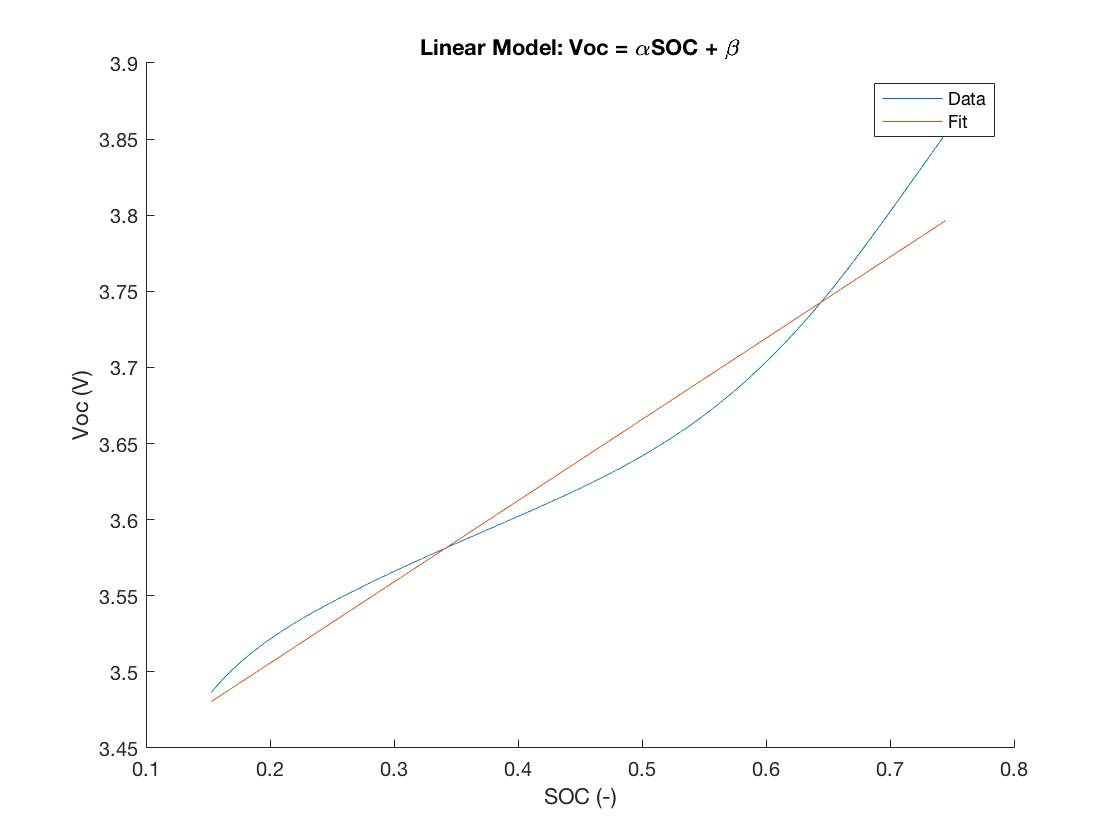
\includegraphics[width=\textwidth]{SOC_Voc.jpg}
\end{figure}

\subsection{}

The equation for the voltage at the terminal of the batteries is as follows:

\begin{equation} \label{}
V_{batt}(t) = V_{OC}(t) - R_0I(t) - V_1(t)
\end{equation}

From the previous part of this problem, we also have: 
\begin{equation} \label{}
V_{OC}(t) = \alpha SOC(t) + \beta
\end{equation}

Plugging in and converting to the frequency domain via Laplace transform:

\begin{equation} \label{}
V_{batt}(s) = \alpha SOC(s) + \frac{\beta}{s} - R_0I(s) - V_1(s)
\end{equation}

However, the derivative of SOC is directly related to input current:

\begin{equation}
\frac{dSOC}{dt} = -\frac{1}{3600Q}I(t)
\end{equation}
\begin{equation}
sSOC(s) = -\frac{1}{3600Q}I(s) + SOC(0)
\end{equation}
\begin{equation}
SOC(s) = -\frac{1}{3600Q}\frac{I(s)}{s} + \frac{SOC(0)}{s}
\end{equation}

The expression for \(V_1\) was derived earlier in the course:

\begin{equation} \label{}
\frac{dV_1}{dt} = -\frac{1}{R_1C_1}V_1(t) + \frac{1}{C_1}I(t)
\end{equation}
\begin{equation} \label{}
sV_1(s) = -\frac{1}{R_1C_1}V_1(s) + \frac{1}{C_1}I(s)
\end{equation}
\begin{equation}
V_1(s) = \frac{R_1}{R_1C_1s + 1}\frac{I(s)}{s}
\end{equation}

Plugging into Equation 3:
\begin{equation}
V_{batt}(s) = -\frac{\alpha}{3600Q}\frac{I(s)}{s} + \frac{SOC(0)}{s} - \frac{\beta}{s} - R_0I(s) - \frac{R_1}{R_1C_1s + 1}I(s)
\end{equation}

In order to solve for the impedance, the terms that do not have I(s) must be ignored. Throwing out these terms yields:
\begin{equation}
Z(s) = \frac{V(s)}{I(s)} = -\frac{\alpha}{3600Q}\frac{1}{s} - R_0 - \frac{R_1}{R_1C_1s + 1}
\end{equation}

\subsection{}
Yes - since we are given the full complex values of Z over the range of the EIS dataset, we can plug into Equation 11 for \(s = j\omega\) and use previous methods like fminsearch or ga to minimize a cost function for the difference between a calculated value of impedance and a measured value of impedance. 

\subsection{}

See code for implementation. The starting values used for the parameters were \(R_0 = 0.03, R_1 = 0.01, C_1 = 1000\) since these were in the middle of the range seen in the midterm data. The lower and upper bounds were \(0.01\cdot\theta_0\) and \(10\cdot\theta_0\). 

\subsection{}

\begin{center}
\begin{tabular}{|c|c|c|}
\hline
Aging Cycle & $RMS(|Z|)$ & $RMS(\phi)$ \\
\hline
1 & 8.67\% & 34.7\% \\
\hline
2 & 5.90\% & 35.3\% \\
\hline
3 & 6.77\% & 39.3\% \\
\hline
\end{tabular}
\end{center}


\subsection{}

\begin{center}
\begin{tabular}{|c|c|c|c|}
\hline
Aging Cycle & $R_0 (\Omega)$ & $R_1 (\Omega)$ & $C_1 (F)$ \\
\hline
1 & 0.0288 & 0.0482 & 1959 \\
\hline
2 & 0.0289 & 0.0100 & 1034 \\
\hline
3 & 0.0318 & 0.0098 & 1082 \\
\hline
\end{tabular}
\end{center}

\pagebreak

\subsection{}

\begin{figure}[h]
\centering
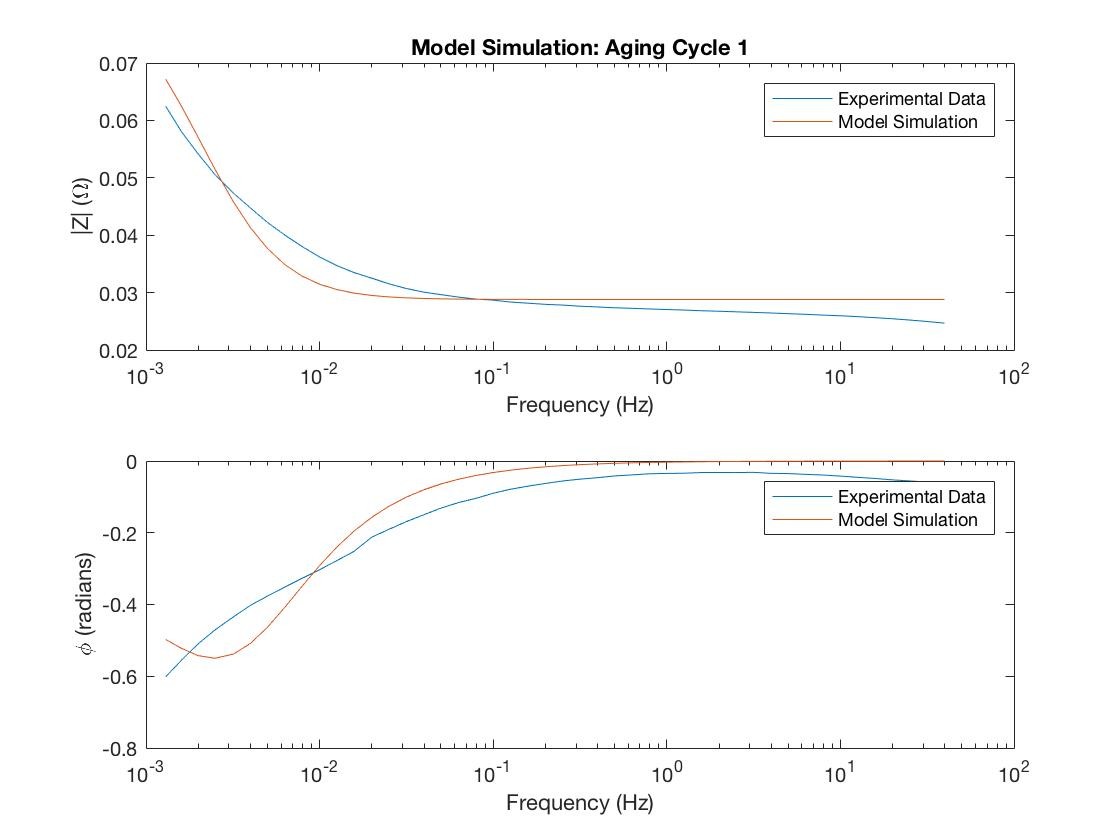
\includegraphics[width=0.8\textwidth]{cycle1_model.jpg}
\end{figure}

\begin{figure}[h]
\centering
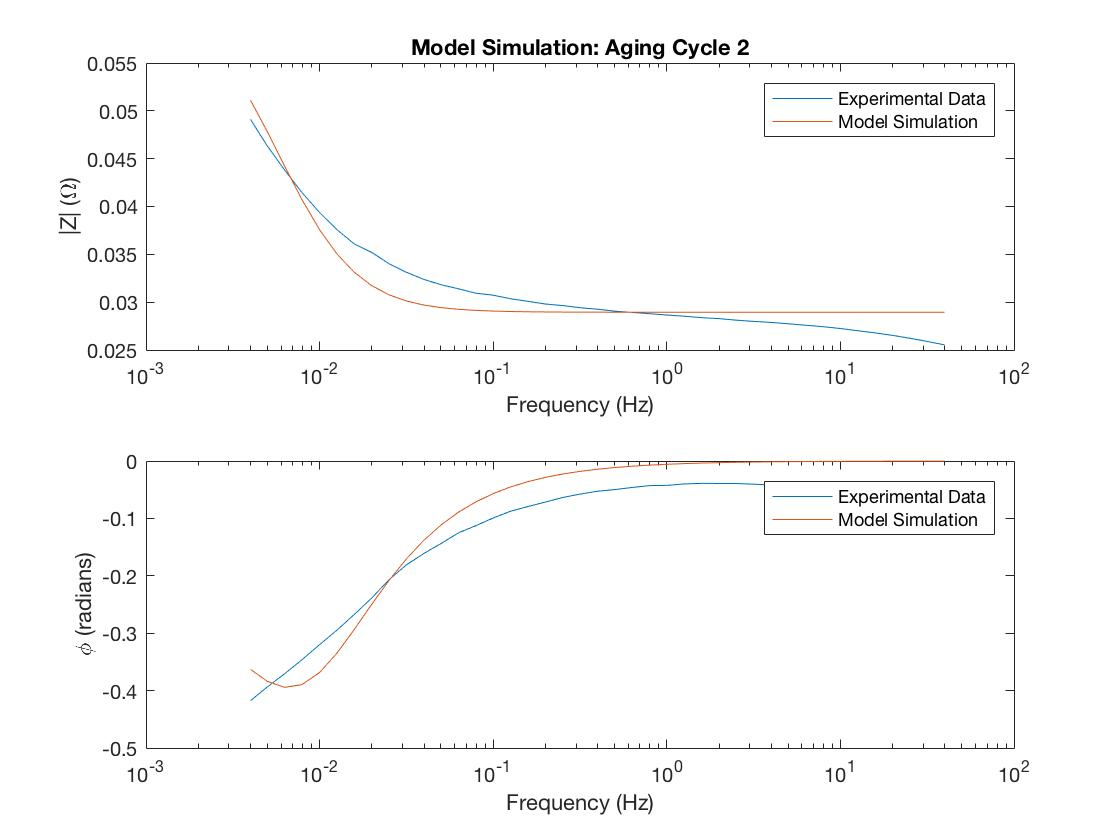
\includegraphics[width=0.8\textwidth]{cycle2_model.jpg}
\end{figure}

\pagebreak

\begin{figure}[h]
\centering
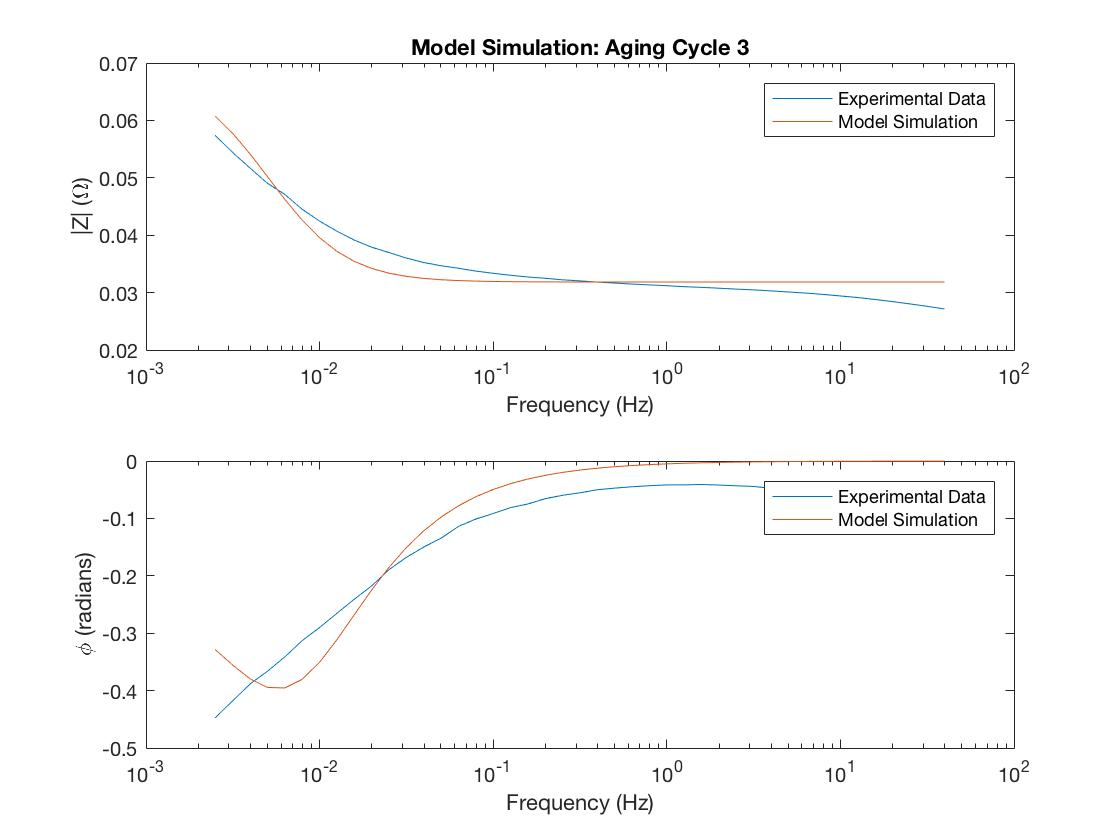
\includegraphics[width=0.8\textwidth]{cycle3_model.jpg}
\end{figure}

\subsection{}

This seems quite different from my intuitions based on the Nyquist plot. The Nyquist plot seemed to show that with increasing age, \(R_E\) would increase slightly, \(R_{CT}\) would increase significantly, and \(C_{DL}\) would increase, if anything. However, the optimal solutions show \(R_0\) increasing slightly, \(R_1\) decreasing, and \(C_1\) decreasing. The results do not match my physical intuition (this may be because I am interpreting the Nyquist plots wrong). However, the RMS is reasonable for the magnitude of the impedance, which is promising. 

\end{document}
